%
% This is the LaTeX template file for lecture notes for EE 382C/EE 361C.
%
% To familiarize yourself with this template, the body contains
% some examples of its use.  Look them over.  Then you can
% run LaTeX on this file.  After you have LaTeXed this file then
% you can look over the result either by printing it out with
% dvips or using xdvi.
%
% This template is based on the template for Prof. Sinclair's CS 270.

\documentclass[twoside]{article}
\usepackage{graphicx}
\usepackage{algorithm}
\usepackage{algpseudocode}
\usepackage{graphics}
\setlength{\oddsidemargin}{0.25 in}
\setlength{\evensidemargin}{-0.25 in}
\setlength{\topmargin}{-0.6 in}
\setlength{\textwidth}{6.5 in}
\setlength{\textheight}{8.5 in}
\setlength{\headsep}{0.75 in}
\setlength{\parindent}{0 in}
\setlength{\parskip}{0.1 in}

%
% The following commands set up the lecnum (lecture number)
% counter and make various numbering schemes work relative
% to the lecture number.
%
\newcounter{lecnum}
\renewcommand{\thepage}{\thelecnum-\arabic{page}}
\renewcommand{\thesection}{\thelecnum.\arabic{section}}
\renewcommand{\theequation}{\thelecnum.\arabic{equation}}
\renewcommand{\thefigure}{\thelecnum.\arabic{figure}}
\renewcommand{\thetable}{\thelecnum.\arabic{table}}

%
% The following macro is used to generate the header.
%
\newcommand{\lecture}[4]{
   \pagestyle{myheadings}
   \thispagestyle{plain}
   \newpage
   \setcounter{lecnum}{#1}
   \setcounter{page}{1}
   \noindent
   \begin{center}
   \framebox{
      \vbox{\vspace{2mm}
    \hbox to 6.28in { {\bf EE 382C/361C: Multicore Computing
                        \hfill Fall 2016} }
       \vspace{4mm}
       \hbox to 6.28in { {\Large \hfill Lecture #1: #2  \hfill} }
       \vspace{2mm}
       \hbox to 6.28in { {\it Lecturer: #3 \hfill Scribe: #4} }
      \vspace{2mm}}
   }
   \end{center}
   \markboth{Lecture #1: #2}{Lecture #1: #2}
   %{\bf Disclaimer}: {\it These notes have not been subjected to the
   %usual scrutiny reserved for formal publications.  They may be distributed
   %outside this class only with the permission of the Instructor.}
   \vspace*{4mm}
}

%
% Convention for citations is authors' initials followed by the year.
% For example, to cite a paper by Leighton and Maggs you would type
% \cite{LM89}, and to cite a paper by Strassen you would type \cite{S69}.
% (To avoid bibliography problems, for now we redefine the \cite command.)
% Also commands that create a suitable format for the reference list.
\renewcommand{\cite}[1]{[#1]}
\def\beginrefs{\begin{list}%
        {[\arabic{equation}]}{\usecounter{equation}
         \setlength{\leftmargin}{2.0truecm}\setlength{\labelsep}{0.4truecm}%
         \setlength{\labelwidth}{1.6truecm}}}
\def\endrefs{\end{list}}
\def\bibentry#1{\item[\hbox{[#1]}]}

%Use this command for a figure; it puts a figure in wherever you want it.
%usage: \fig{NUMBER}{SPACE-IN-INCHES}{CAPTION}
\newcommand{\fig}[3]{
			\vspace{#2}
			\begin{center}
			Figure \thelecnum.#1:~#3
			\end{center}
	}
% Use these for theorems, lemmas, proofs, etc.
\newtheorem{theorem}{Theorem}[lecnum]
\newtheorem{lemma}[theorem]{Lemma}
\newtheorem{proposition}[theorem]{Proposition}
\newtheorem{claim}[theorem]{Claim}
\newtheorem{corollary}[theorem]{Corollary}
\newtheorem{definition}[theorem]{Definition}
\newenvironment{proof}{{\bf Proof:}}{\hfill\rule{2mm}{2mm}}

% **** IF YOU WANT TO DEFINE ADDITIONAL MACROS FOR YOURSELF, PUT THEM HERE:

\begin{document}
%FILL IN THE RIGHT INFO.
%\lecture{**LECTURE-NUMBER**}{**DATE**}{**LECTURER**}{**SCRIBE**}
\lecture{1}{August 24}{Vijay Garg}{Rahul Jaisimha}
%\footnotetext{These notes are partially based on those of Nigel Mansell.}

% **** YOUR NOTES GO HERE:

% Some general latex examples and examples making use of the
% macros follow.  
%**** IN GENERAL, BE BRIEF. LONG SCRIBE NOTES, NO MATTER HOW WELL WRITTEN,
%**** ARE NEVER READ BY ANYBODY.
\section{Introduction}

This class was just an introduction to the course. It explained how to write concurrent programs using the different framework/languages we will be using in class. All files used in this lecture can be found in the {\tt chapter1-threads} folder of the class github \cite{1}.

\section{First Things First}

Dr. Garg's office is a gun-free zone.

\section{Writing Concurrent Programs}

\subsection{Java}

See github file {\tt java/HelloWorldThread.java}. Concurrent programming in java is implemented by extending the {\em Thread} class in java and overriding the {\tt run()} function. {\tt thread.start()} is used to start the thread.\\
This program can be run on Unix with:\\
{\tt javac HelloWorldThread.java}\\{\tt java HelloWorldThread}

\subsection{OpenMP}

See github file {\tt openMP/hello.c}. Concurrent programming using openMP is implemented by including {\tt omp.h} and using {\tt -fopenmp} as an argument during compilation (as seen in compile.bat also on github). Use {\tt \#pragma} to run things in parallel. In {\tt hello.c}, every thread should have a private copy of {\tt tid}.

\subsection{Pthreads}

See github file {\tt pthreads/hello.c}. This is the longest program. Compilation is normal unlike openMP. The program just has to include {\tt pthread.h}. 

\subsection{Promela}

See github file {\tt spin/helloThreads.pml}. The program starts at {\tt init} much like {\tt main()} in other languages. Input the promela file and properties into {\em Spin} to run.\\
This program can be run on Unix with:\\
{\tt spin helloThreads.pml}

\subsection{Cuda}

See github file {\tt cuda/hello.cu}. Cuda is used to write GPU programs. More on Cuda programming in the next section.


\section{GPU Programming}

GPGPU = General Purpose GPU. GPGPUs are useful for matrix multiplication, neural networks, amongst other things.
GPU programming relies on SIMD (Single Instruction Multiple Data). This means programming multiple processes to do the same thing on different data.

\begin{figure}[h!]
\centering
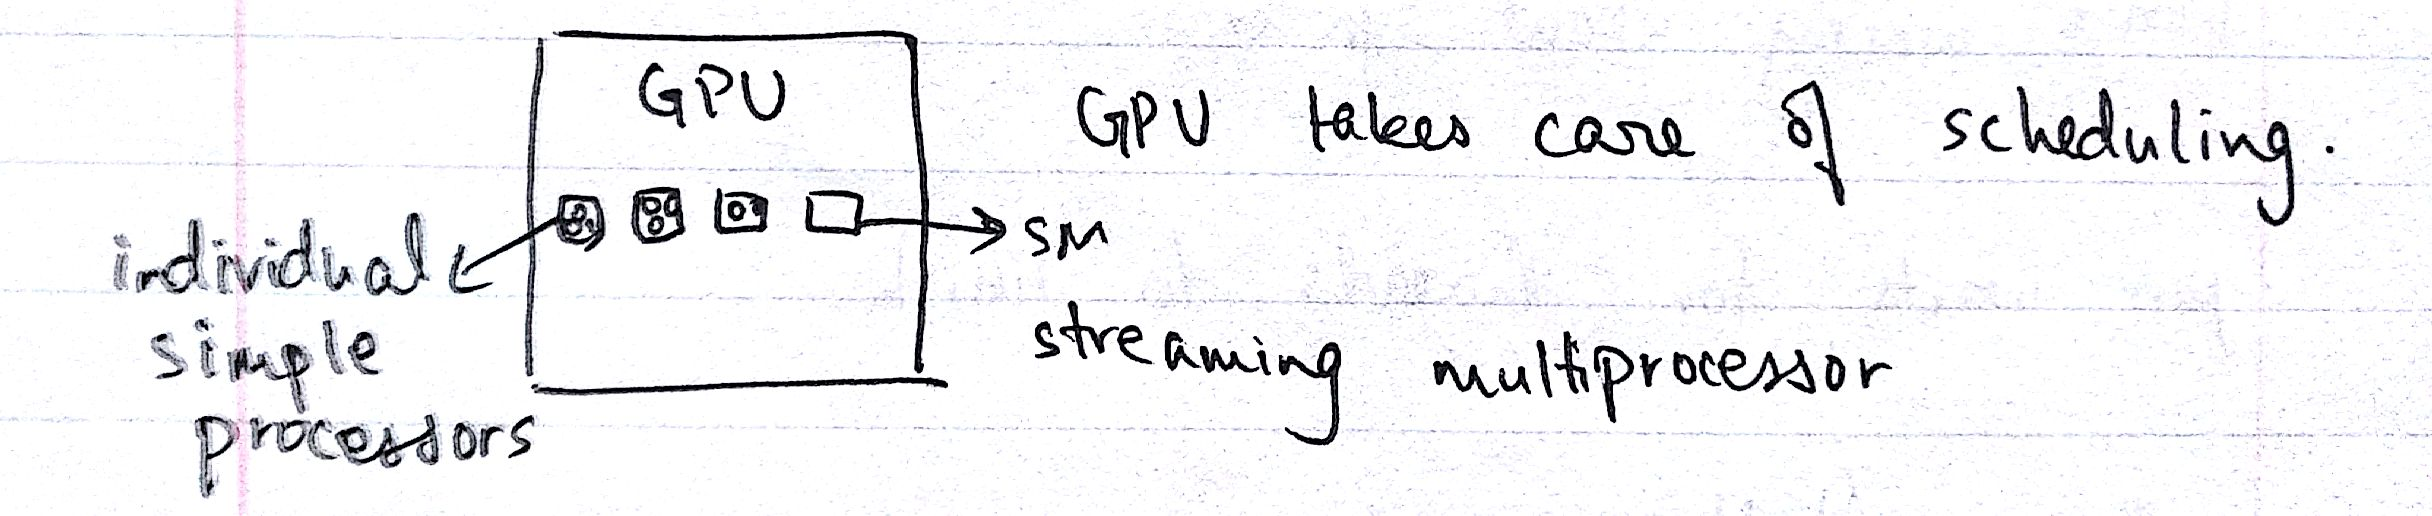
\includegraphics[width=150mm]{gpu}
\caption{GPU}
\label{fig:method}
\end{figure}

\subsection{Cuda cont'd.}

Cuda uses the notion of kernel. the {\tt \_\_global\_\_} is used to denote running on the gpu. Cuda programs are compiled with the Nvidia Cuda compiler {\tt nvcc}.
Note that optimizing GPU programs is a lot harder than optimizing CPU programs.

\section{PRAM}

PRAM = Parallel RAM. PRAM is purely an abstract concept for developing parallel algorithms that assumes shared memory between many processing elements.

\begin{figure}[h!]
\centering
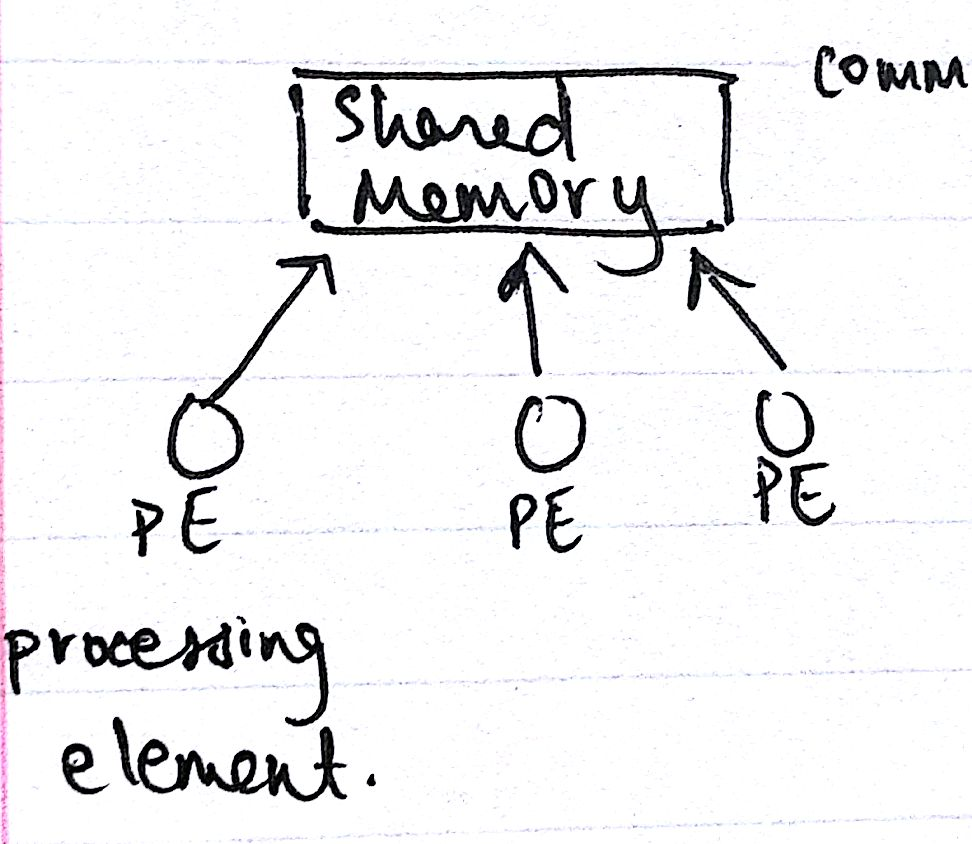
\includegraphics[width=80mm]{pram}
\caption{PRAM}
\label{fig:method}
\end{figure}

Algorithms for accessing the shared memory from each processing element are either of CRCW, CREW, ERCW, or EREW. E: Exclusive, C: Concurrent, R: Read, W: Write.

\section{The Dr. Garg Traditional First Day of Class Puzzle}

Assume you have an array of unique natural numbers (non-negative numbers). Let its size be $N$. Find the largest element in the array.\\
In this section we use work complexity to denote number of compares. We also assume we have $N^2$ cores (or as many cores as we need).

\subsection{Sequential Algorithm}

Time Complexity = $O(N)$\\
Work Complexity = $O(N)$\\
Cores needed = 1

\subsection{Binary Tree Algorithm}

Split the array into a binary tree and compare two at a time recursively.\\

Time Complexity = $O(\log N)$\\
Work Complexity = $O(N)$\\
Cores needed = $N$

\subsection{"Usain Bolt Algorithm"}

\begin{algorithm}
    \begin{algorithmic}[]
	\State $\forall i, isBiggest[i] := 1$
        \ForAll{$i, j$}
	    \If{$A[j] > A[i]$}
            	\State $isBiggest[i] \gets 0$
	    \EndIf
        \EndFor
	\If{$isBiggest[i]$}
	   \State $MAX := A[i]$
	\EndIf
    \end{algorithmic}
    \caption{"Usain Bolt algorithm"}
\end{algorithm}

Time Complexity = $O(1)$\\
Work Complexity = $O(N^2)$\\
Cores needed = $N^2$

\subsection{Epilogue}

Okay so that was pretty good, but can we solve this problem with a good time complexity like $O(\log N)$ without using so many cores?

\section*{References}
\beginrefs
\bibentry{1} https://github.com/vijaygarg1/UT-Garg-EE382C-EE361C-Multicore/tree/master/chapter1-threads
\endrefs


\end{document}





